\documentclass[12pt,a4paper,titlepage]{article}

\usepackage{times}
\usepackage{setspace}
\usepackage{textcomp}
\usepackage[a4paper,left=1in,top=1in,right=1in,bottom=1in]{geometry}
\usepackage{graphicx}
\usepackage{caption}

\usepackage[english]{babel}
\usepackage[backend=bibtex]{biblatex}
\usepackage{csquotes}

\usepackage[bookmarks]{hyperref}
\hypersetup{colorlinks=true,allcolors=black}
\usepackage{hypcap}


\bibliography{sources}


\doublespacing{}
\oddsidemargin = 0pt
\headheight = 0pt
\topmargin = 0pt
\headsep = 0pt
\marginparwidth = 0pt
\textwidth = 450pt


\begin{document}

\title{Apple Inc.}
\author{Kevin Bloom \\ MET315--02}
\maketitle

\newpage

\pagenumbering{roman}
\tableofcontents

\newpage

\pagenumbering{arabic}

\section{Description of Company}
Apple is one of the most successful companies of all time. Not only in the
U.S. but in the whole world. They are one of the biggest designers/manufacturers
of desktops, laptops/netbooks, tablets, and smartphones as
well~\cite{hoover}. Not to mention their massive grip on the multimedia realm
with iTunes, Apple Music, Apple TV, and their assortment of multimedia editing
programs. They don't only rule the school of multimedia, however. They are
rapidly seizing the tech world due to its easy-to-use interface and unix-based
(DarwinOS) background. Monetarily, the company does extremely well; as would any
company among the top in the world. Just one of their products, the iPhone, is
responsible for two-thirds of the company's revenue~\cite{hoover}. This may not
be too surprising because pretty much \emph{everyone} has an iPhone! That being
said, Apple's biggest claims to fame are as a computer hardware/software
manufacturing/designing company and as a catalyst of new technology in the
market.

Mostly everyone has heard of the founders Steve Jobs and Steve Wozniak. Wozniak
left the company in 1983, only 3 years after the company went
public~\cite{hoover}. Jobs was with the company on and off\footnote{In 1985,
  Jobs resigned from Apple due to workplace drama with John Sculley. He rejoined
  Apple in 1997~\cite{jobs}.} until his death in 2011. After his death, Tim Cook
took over as CEO and remains to this day. A few other notable employees of the
company are: Dr. Arthur Levinson, chairman, Jeff Williams, COO, Jonny Ive, chief
design officer, Craig Federighi, SVP software engineer, Dan Riccio, SVP hardware
engineer, and Phil Schiller, SVP worldwide marketer~\cite{hoover}. We know most
of these people from Apple's events which they come on stage to talk. Jonny Ive
is most known for the videos that reveal the newest Apple projects. Either way,
without these people, and many more, Apple would not be as successful as it is
today.

Most people know that Apple doesn't assemble most of their devices in the
US. How do they know this? Well, on the back of any Apple device, there will be
a note informing the user that it was designed in the US but assembled in
China. According to LexisNexis Academic, they have a subsidiary called
\emph{AuthenTec}. One of the locations for this company is in Shanghai, which I
believe is the main manufacturing plant for some of their bigger
products~\cite{lexis}. That being said, there are also some plants/facilities
found in Japan, Mexico, Europe, and even Australia~\cite{lexis}. Their
headquarters is located in Cupertino, Califonia and is approximately 16,000
sq. ft in size~\cite{hoover}. Apple has hundreds of locations all over the
world, ranging from design facilities to retail stores to manufacturing.

Needless to say, Apple does a lot of business. They sell a lot of product. In
fact, in 2016 they had about \$215,639,000 worth of sales~\cite{hoover}!  Also
according to Hoover, they have a market value of about \$594,339,610. Talk about
big numbers! Apple sold approximately 226,200,000 iPhones~\cite{lifewire} and
about 45,590,000 iPads~\cite{lifewire2} in 2016 alone. Just based on those
approximate numbers, we can determine that Apple gets all most all of it's
revenue from the iPhone. Let's not forget the other slew of products they sell
that weren't mentioned. That being said, the volume of product from Apple is
absolutely enormous! Along with their huge fan base, it's no wonder they are so
successful.

\newpage

\section{Stock Chart}

\begin{figure}[!htb]
  \centering
  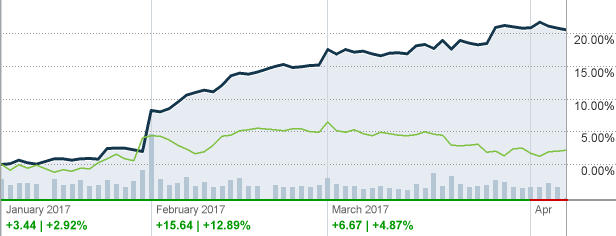
\includegraphics[width=1\textwidth]{apple-chart-3mo}
    \caption{Apple (blue) vs NASDAQ (green) for 3 months~\cite{cnnapple}}
\end{figure}


\begin{figure}[!htb]
  \centering
  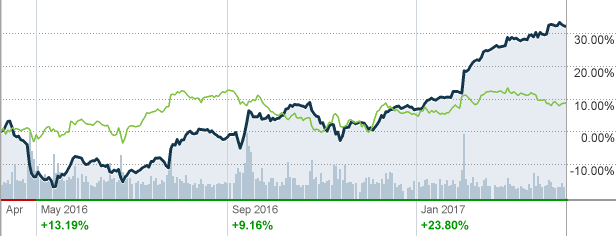
\includegraphics[width=1\textwidth]{apple-chart-1yr}
    \caption{Apple (blue) vs NASDAQ (green) for 1 year~\cite{cnnapple}}
\end{figure}

\begin{figure}[!htb]
  \centering
  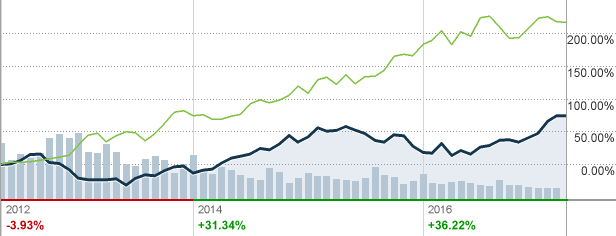
\includegraphics[width=1\textwidth]{apple-chart-5yr}
    \caption{Apple (blue) vs NASDAQ (green) for 5 years~\cite{cnnapple}}
\end{figure}

\newpage

\section{Discussion of Chart}
In the figures found on the previous page, you will notice that I chose to
compare Apple to the NASDAQ for the past 3 months, year, and 5 years. Firstly,
my reasoning for choose NASDAQ was simple; I felt as though it would give a
good visual as to how the market as a whole was doing. Secondly, I selected
multiple graphs so that I could analyze the company for longer than just the
required period; not to mention the \emph{Financial Performance} section has to
do with the past 5 years. Now that the preliminaries are out of the way, let the
discussion begin!

While looking at the graphs, one would notice that Apple seems to be doing quite
poor in comparison to the NASDAQ; except for the past 2 months (Feb. through
Apr.). For the past years, Apple has been dancing around the NASDAQ, as seen in
Figure 2. During spring-summer months, Apple tends to do poorly because they
don't have anything huge being released. iPhones tend to be released in
September and, as we saw earlier, is their biggest seller. This would explain
how, in Figure 2, Apple jumps up to about even with the NASDAQ. The new iPhone
would then ride the company through Christmas and into the new year. This
doesn't explain why they are 20\% above the NASDAQ from February until
now. Well, it looks as though the company had it's best holiday quarter ever in
2016~\cite{fool}. Also according to The Motley Fools, ``their fast-growing
service segment ... has expanded to nearly 10\% of sales, and soaring demand for
apps pushed its high-margin revenue.'' This very well could explain that large
jump, meaning that the company is doing well right now.

The last thing to discuss is the company's 5 year graph. In 2012, Apple was
about fair with the NASDAQ. Then the NASDAQ started to move away, and never
crossing paths again until this year. I found this rather interesting but I
believe that the reasoning for this is that Apple has a safety net. The company,
although very intuitive, doesn't make extreme changes on their
products.\footnote{Besides them removing the 3.5mm headset jack on their newest
  model iPhone.} This gives the customer a sense of home, even when they get a
new device. While they are doing that, the market is trying all sorts of new
things. Since the NASDAQ doesn't solely rely on Apple, it might have to do with
other companies making more galvanizing devices that caused the NASDAQ to leave
Apple in the dust.

\section{Financial Performance}
Information I will be discussing in this section can be found in Section 11,
which are sections from Apple's financial records. They each contain the past 5
years. Starting with the balance sheet, you will find the assets table
first. The very first thing to note is that 2016 seems to have the biggest
numbers in almost all the categories; some even being significantly larger. For
example, their total current assets is up from 2015 by about 17,491 million,
total assets are up 31,207 million, and cash/equivalents are up 25,554
million. There doesn't seem to be any major decreases, which is good. There
aren't many major drops, except the drop in other current assets by 6,502
million. Overall, this part of the balance sheet looks good and points the
company toward a successful direction.

Looking at the next piece of the balance sheet is the liabilities. The only
thing that I'm going to note is that the total liabilities seem to be increasing
with time. This isn't necessarily a bad thing, but it isn't necessarily a good
thing either. Luckily, their total assets is significantly greater than their
total liabilities. So far the company seems to be holding up well on their
balance sheet. Let's look into the income and cash flow statements.

The income statement is found in Section 11.2 (Income Statement). The very first
thing I noticed was that 2016 dropped by about 10,000 million in almost every
category. In fact, the sales dropped by about 15,000 million. Another
interesting thing to note is that 2015 has the highest numbers for all the years
listed. Luckily the cost of goods also dropped as well, saving the company some
money. The numbers dropped, but they didn't drop below any previous year, which
is good. Overall, it's bad that it dropped, but nothing too scary yet. The cash
flow statement, found in Section 11.3 (Cash Flow Statement), supports the same
claim, for the most part. It seems as though they increased the number of
operating activities\footnote{This could be because of their iPhone recycling
  campaign, if so, that's a warm fuzzy to consider.} and dropped
investments. In this case, some of the values dropped below previous years,
but, yet again, this isn't something to worry about too much. Overall, I believe
that the company is growing, despite having a couple small set backs. I believe
this because the company's numbers are still high and haven't dropped too
low. However, it's still very important that they keep it up or they could be in
trouble.

\newpage

\section{Performance Ratios}
All of the ratios I will be discussing in this section will be coming from
Zack's balance sheet and income statement found in section 11. My calculations
are found in Appendix B. First and foremost, you will notice that Apple's PE
ratio for all five previous years have been fairly close. They aren't extremely
small, but I suppose they could be higher. In the grand scheme of things, I
believe this is a fairly good stock; for all of the years. Their current ratio
is also good because it is greater than 1. They did get very close to 1 in 2015
and 2014 but looks like they're going up. Throughout the years listed, Apple
seems to have an alright quick ratio as well. It only dropped under a dollar for
2 years, 2015 and 2014, and seems to be going back up. Although these number are
best when higher, they aren't terrible, for the most part.

We've looked at the company's ability to pay off their debt, now let's look at
their actual debt. According to my calculations, about 60\% of the company is
debt to others currently. This is quite the percentage! As I expected, the
percent is going up with the years due to their ever increasing costs. In 2012,
the company was only about 33\% debt which means that it increased its debt by
about 30\% in 4 years. I don't really find this all that surprising coming from
Apple, but 60\% is a lot of debt. Looking back at their current ratio, the
company does have the ability to pay back their current debt. This may mean that
they also have the ability to pay back there long term debt. Either way, let's
look more into their ratios to see if we can unwrap this mysterious case.

To my surprise, the working capital wasn't extremely large;\footnote{Don't get
  me wrong, it was \emph{large} just not to the extreme} especially in 2014 and
2015. Once again we see the same trough in those years and Apple come out of it
in 2016. In fact, the working capital more than tripled from 2015! As discussed
earlier, 2016 was when Apple started to meet up with the NASDAQ in the stock
market. This obviously means that 2016 was a very important time for the
company. While on the topic of dollar amounts, their new worth is fairly
consistent with the rest of the data. Once again, there was a drop in 2014 and
2015 and an increase into 2016. The drop is about 10,000 million, which is
significant. It's a good thing that they got out of that trough.

Looking at the return on assets for Apple, I noticed that early on was
better. 2013 and 2012 both had high number, meaning that their assets must
having been making very good profit. Contrary to the past situations, 2015 and
2014 didn't prove to be terrible for ROA, in fact, they were about average for
the company during these 5 years. In terms of return on equity, there isn't much
change. Oddly enough, their returns are pretty constant throughout the five
years. The maximum was in 2012 and the minimum in 2015. Not too much to say
here. Lastly, their return on sales for the most part are constant throughout
the 5 year range. The only exception is for 2016, where the ROS dropped by about
15\%. This could mean that Apple didn't use their assets very wisely in that
year. Overall, their return numbers are excellent for the most part.

The last ratios I will be discussing are the profit margins. Their PM before
taxes throughout the 5 years were consistent. There weren't any huge drops or
increases. The same can be said about the PM after taxes. In fact, the
difference between the PBIT and PAIT isn't very big at all, maxing out around
9\% in 2012. On average the company seems to be making about 20-30\% profit
after taxes. Overall, you can see that Apple's performance is great. There are
only a few areas in which I'm a little unsure about, namely, their
debt. However, with Apple's strong hold on the market, I don't think this will
be a big issue.

\newpage

\section{Positives \& Negatives}
From the last section, I found out a lot of information about Apple that could
be seen as positive or negative. Starting with the positives, the company seems
to have a decent current ratio. This means the company is able to pay off their
current debt. Another positive factor from their performance is that they have
a decent net worth. They also have very stable profit margins. Out of all the
information given, I believe that the most important piece to the puzzle is that
the company is able to get themselves out of trouble. We saw how they dropped in
2014 but they returned stronger than ever in 2016. We could also see this
on the stock graphs from earlier. The company seemed to be behind the NASDAQ yet
came back with vengeance in 2016. I believe that this is the most positive thing
that Apple has going for them financially.

Apple is doing very well in their sector. As you will see in the
\emph{Competition} section, Apple is pretty much on top in the smartphone and
laptop industry. These are Apple's primary markets, so doing well in the means
that the company is doing it's job right. Just comparing the revenue of their
top competitors we can see this. Apple is at about \$215 million right now while
Amazon is at \$107 million, Google is at \$75 million, HP is at \$103 million,
and Samsung is at \$170 million. There is only 1 company on Hoover's profile for
Apple that has a revenue great than Apple's, and that's Wal-Mart. It's obvious
to see that Apple isn't joking around when it comes to competition.

The financial negatives that I saw from Apple were simple: debt. The company
seems to have a large debt. From my calculations, it's about 60\% of the
company. This is a very large amount of debt that would make me feel
unconformable if I were running the business. However, this information is from
2016 and we are well into 2017. The company could have, at this point, paid some
of that debt off. Since we saw that they have a decent current ratio, this could
be possible.\footnote{I'm aware that CR has to do with \emph{current} debt, not
  long term, but I would imagine that a company whom can pay off current debt,
  can probably pay off long term for the most part.} As mentioned before, I
don't truly know if this debt would be consider an actual issue for the company
givens its position on the market. I'm sure that their people are well aware of
the deficit and are working on ways to lower it, without costing the company
valuable product quality.

\newpage

\section{Non-Financial Concerns}
Most people know that Apple is always suing someone. Recently, Apple has been
having issue with it's competitor Samsung. Most notably due to Apple's claim
that Samsung copied the iPhone for their Galaxy S series of smartphones. In
fact, the case regarding this dispute was reopened \emph{this
  year}~\cite{sue}. In fact, Apple has quite a few lawsuits going on right
now. Some of which are with Swatch, Qualcomm, and Nokia~\cite{insider}. A
company with that many lawsuits seems a little odd, don't you think? I believe
there are a lot of people that don't like Apple because of their constant
lawsuits.

There are many people that specifically don't use Apple's products.  One of
those groups is called the Free Software Foundation. This group of freedom
fighters have some major issues with most computer companies but they
specifically have beef with Apple. They claim that Apple's operating systems
have back doors, censorship systems, digital rights management (DRM), and many
more malicious features~\cite{gnu}. As a member of the foundation, I know that
what they speak about is most likely true. We have found many systems to be
malicious before; mostly for the benefit of the company. Either way, having
these features is something that most people don't want. This could (and does)
deter people from purchasing Apple's products.

Enough of the bad stuff, let's look at one of Apple's biggest non-financial
pros: environment. Apple is a company that is devoted to bringing products that
meet all of the environmental standards such as removing poisonous metals from
their devices~\cite{apple-green}. Not to mention that they released their new
iPhone recycling robot, Liam. This machine takes apart all of the iPhone into
it's different components; which can then be properly recycled to make the new
batch of iPhones or other products~\cite{apple-green}. This is one of Apple's
best traits and I think many other agree with me.

\newpage

\section{Competition}
According to Hoover's profile, some of Apple's top competitors are Blackberry,
Google, and HP. Well, this doesn't really seem right to me. In terms of net
gross revenue, Blackberry isn't very high; therefore, I don't really think that
Blackberry is that dangerous of a competitor to Apple. Amazon, Google, HP,
Microsoft, and Samsung are the ones that I would think matter most to
Apple. Coincidentally, Hoover has a different answer to this question not found
in their document for Apple. According to their site, Apple's top competitors
are HP, Samsung, and Google~\cite{hoover-com}. This makes more sense, so let's
go with that!

Both Samsung and Google compete with Apple in the art of smartphones. Samsung is
the runner up in the current mobile market with it's Galaxy S series. According
to DeviceAtlas, the iPhone creams Galaxy devices in terms of global
popularity~\cite{smartphones}. In most countries, listed the iPhone was
the first three most popular devices~\cite{smartphones}.\footnote{Obviously
  different models of the iPhone.} Need I say more? Google is another mobile
competitor of Apple but not in the same way that Samsung is. Google competes
directly with iOS, the iPhone's operating system (OS), with their own OS called
Android. In this race, it's not so obvious as to whom the winner is. I looked at
2 different websites that had polls regarding this topic and both showed that
people prefer Android over iOS about 60:40~\cite{poll1}~\cite{poll2}. The truth
of the matter is that most people like their iPhone because it's easy to use,
reliable, and gets the job done. That being said, these people may not be
considered ``techy'' and wouldn't be going on a technical site to take a
poll. Yes, there are a lot more Android phones on the
market\footnote{Approximately 81\% of the market is Android~\cite{verge}.} but
quantity isn't always better than quality.

The last company to compare to is HP which is in competition with Apple's Mac
lineup. As I expected, HP isn't doing that well in comparison to Apple. The
reason I expected this is because I haven't seen someone with an HP laptop in
years. I never hear about them anymore! Alas, HP comes in 6th place in
WorldsTopMost.com's survey; Apple leading the scoreboard~\cite{most}. I really
don't think that HP is a threat to Apple's Mac lineup. I've noticed lot of
programmers nowadays choose Mac over Windows due to it being UNIX-based and, of
course, Mac has all the multimedia people. Can Apple ever be defeated?

\newpage

\section{Other Information}
There are a lot of interesting things that I didn't discuss that make Apple an
different company. As mentioned earlier, the Free Software foundation is a group
of people that act against the evils of Apple. What's interesting about this
situation is that Apple actually has a lot of free/libre (open source) software
found within their systems~\cite{open-apple}. In fact, the base system of MacOS
is free/libre being based off of FreeBSD. It's mostly the user applications,
drivers, and firmwares that people are upset about. I find this very interesting
that, many people in the free/libre and open source software community dislike
Apple. This could be one of the reason as to why programmers seem to be
switching over to Mac. On top of Apple having a semi-open OS, they also
contribute to many free/libre projects~\cite{open-apple}. Very important
projects such as WebKit, Swift, CUPS~\cite{cups}, and
LLVM~\cite{open-apple}. WebKit, CUPS, and LLVM are projects that many people,
including those in the Free Software Foundation, use on any given day. Needless
to say, Apple has a love/hate relationship with these communities and seem to be
getting more and more involved with them lately.

Another, completely unrelated, topic about Apple that I didn't discuss was their
involvement with the encryption case last year. The FBI wanted access to a
user's iPhone, but they were unable to because of the encryption on the
device. In the attempt to break into the device, they asked Apple to help
them. Apple denied them service, shocking not only the FBI but the entire
world~\cite{cnbc}. In my opinion, this is something that is extremely
important. What this shows is that Apple isn't going to give up people's data;
not event to the FBI. This is a very good thing. Even though we know that
Apple's software isn't the best for our freedom, it is still very good to
know~\cite{gnu}. That being said, this sounds contradictory from what we learned
about Apple's maliciousness in software. It's important to note that although
Apple may have malicious features in their products, they are most likely
\emph{not} selling this information to the government or other companies. This
leaves us with one final question: What \emph{are} they doing with it?

\newpage

\section{Conclusion}
Apple is a company that is good at what it does. They try to keep their products
similar yet different from the previous model. This is something that its
customers both love and hate at the same time. The more ``techy'' people hate
the fact that the newest iPhone looks so similar to last years model while
others love it's simplistic design. If Apple keeps this up, I believe that they
will be in relatively good shape for the next 1-5 years. However, this isn't all
they have to do. If they just do the same old dog and pony show for the next 5
years, things could go awry. I believe that they need to have a good mixture of
innovation with new technology and currently accepted ideas. The numbers have
shown that having the most advanced, crazy technology doesn't always
win. Instead, something with a simple approach and a hint of new age technology
seems to work very well. If you make some technical people unhappy, whatever,
there are more nontechnical people that will be happy.

One thing that especially makes me nervous is the company's large debt. I think
it would be a good idea to try and reduce it as quickly as possible. Without
causing a drop in the quality of company's products. Not to mention the company
needs to be able to keep up with a large amount of product it must output. How
will they do something like this? I'm not sure. With all of the different things
that the company produces, I'm sure there have to ways to cut cost so that they
can put money into paying off the debt. I could be wrong of course and the
company could be secretly being destroyed from the debt.

One last thing that I think the company should keep doing is being a leader in
environmentally friendly computing. I think that this is something that puts
Apple above most other companies. A lot of people admire that they take the time
to make sure that their products are clean and safe for the people that use them
and the environment they may be left in. Not to mention their new recycling
program for iPhones. It would be nice to other ones for their other products. In
the end, I believe that Apple has a bright future ahead.

\newpage

\section{Required Documents}
\subsection{Balance Sheet}
\begin{figure}[!htb]
  \centering
  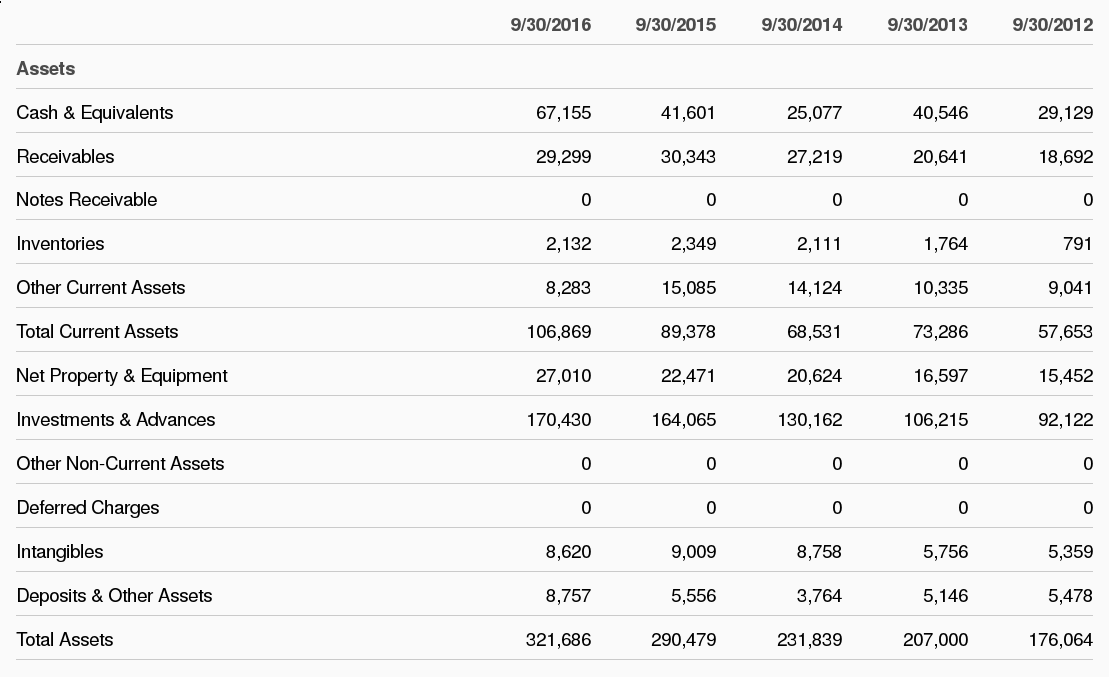
\includegraphics[width=1\textwidth]{assets}
    \caption{Assets. All values in millions except per share data~\cite{zacks-bal}}
\end{figure}

\begin{figure}[!htb]
  \centering
  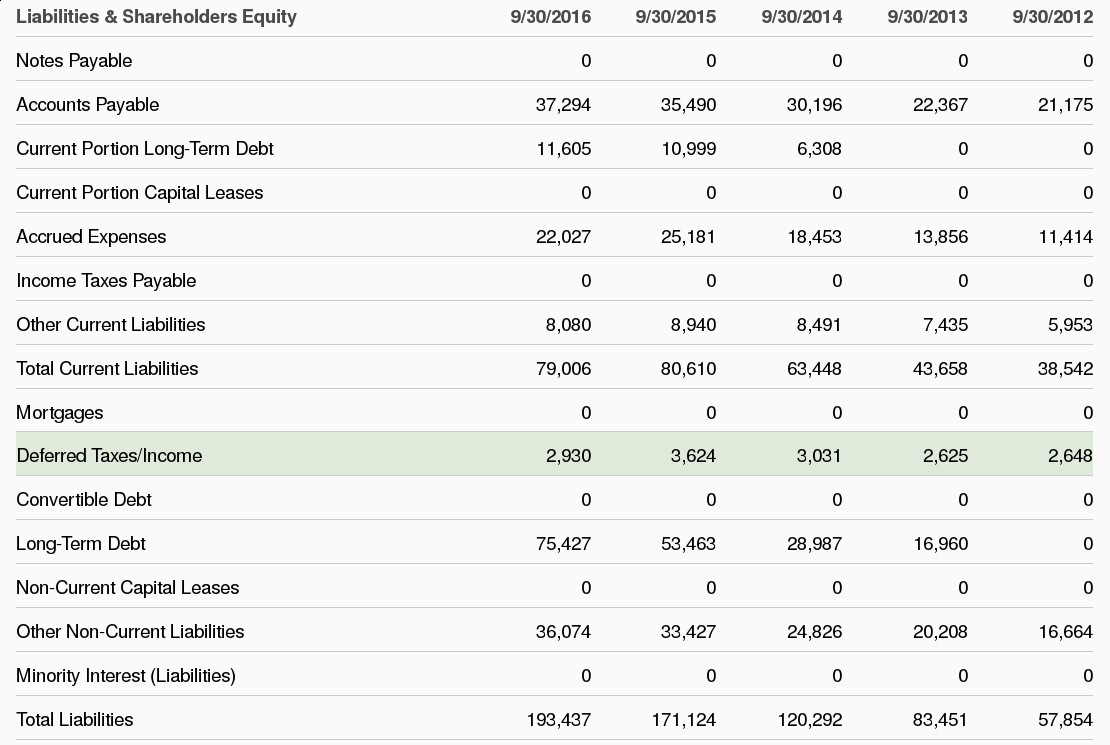
\includegraphics[width=.9\textwidth]{liabilities}
    \caption{Liabilities \& shareholder equity. All values in millions except
      per share data~\cite{zacks-bal}}
\end{figure}

%% \newpage                        %need for formatting

\begin{figure}[!htb]
  \centering
  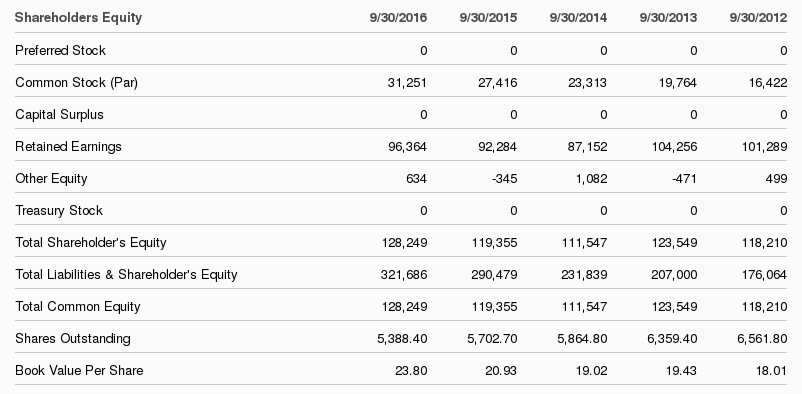
\includegraphics[width=1\textwidth]{shareholder}
    \caption{Shareholder equity. All values in millions except per share
      data~\cite{zacks-bal}}
\end{figure}

\newpage                        %need for formatting

\subsection{Income Statement}
\begin{figure}[!htb]
  \centering
  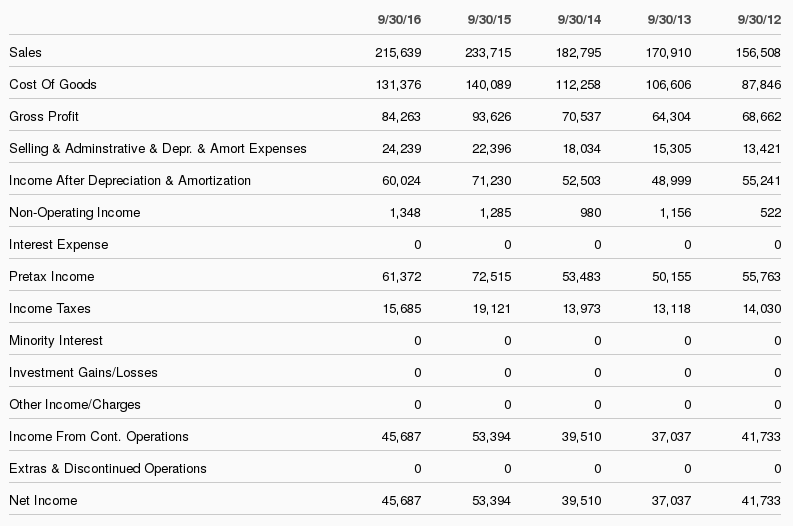
\includegraphics[width=1\textwidth]{income}
    \caption{All values in millions except per share data~\cite{zacks-income}}
\end{figure}

\newpage

\subsection{Cash Flow Statement}
\begin{figure}[!htb]
  \centering
  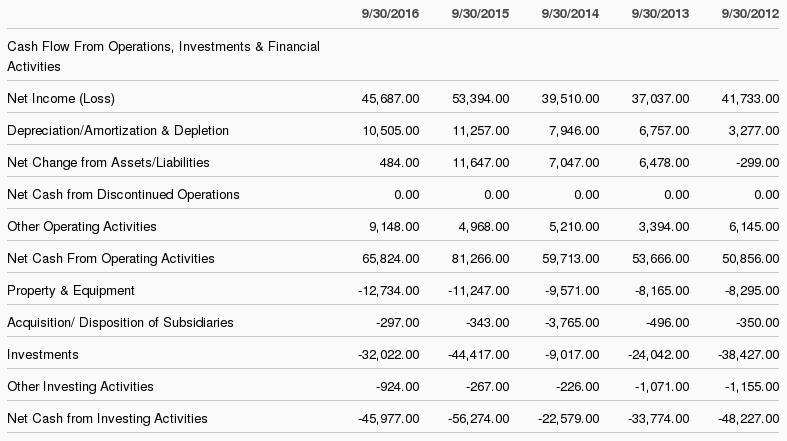
\includegraphics[width=1\textwidth]{cash-flow}
    \caption{All values in millions except per share data~\cite{zacks-cash}}
\end{figure}

\newpage

\appendix

\section{Company Information}
\begin{figure}[!htb]
  \centering
  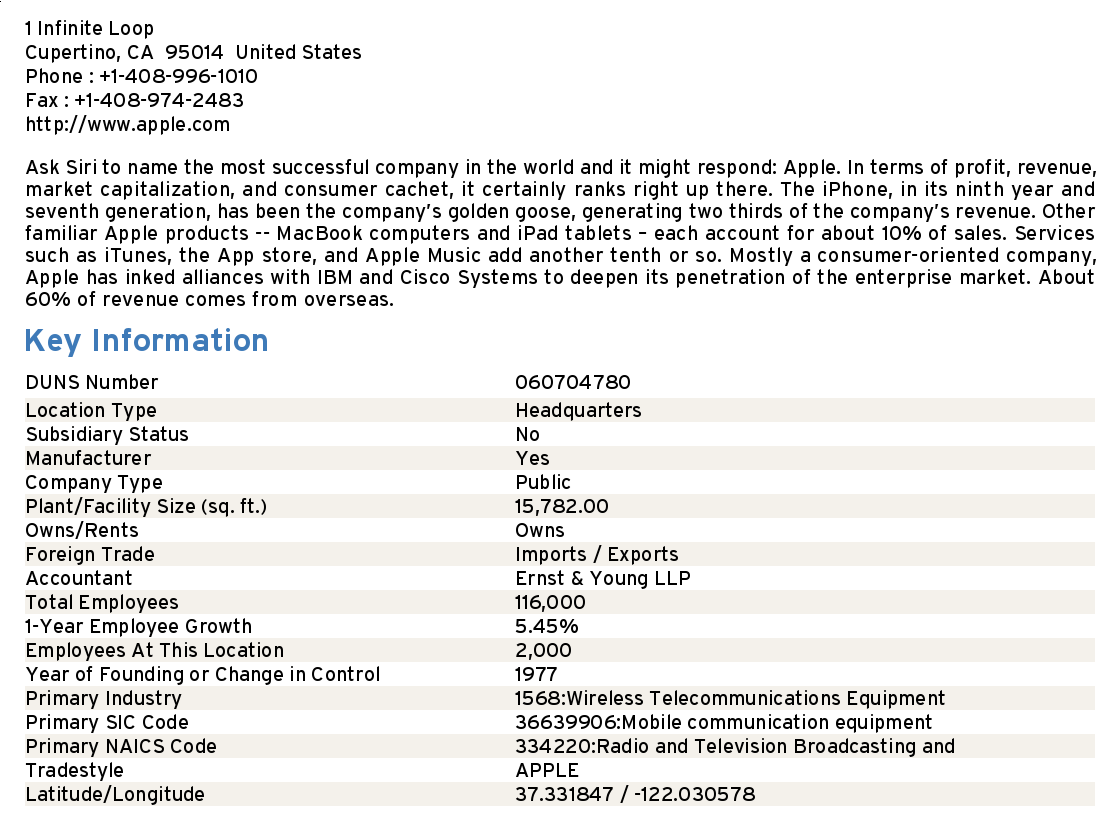
\includegraphics[width=1\textwidth]{overview}
    \caption{Headquarters information. Taken directly from Hoover~\cite{hoover}}
\end{figure}

\begin{figure}[!htb]
  \centering
  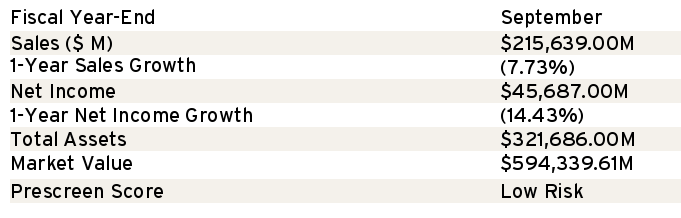
\includegraphics[width=1\textwidth]{keyfin}
  \caption{Key Financials. Taken directly from Hoover~\cite{hoover}}
\end{figure}

\begin{figure}[!htb]
  \centering
  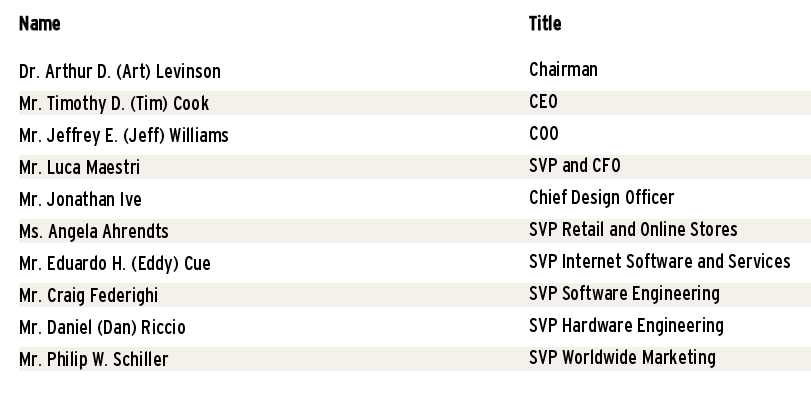
\includegraphics[width=1\textwidth]{employ}
  \caption{Key Employees. Taken directly from Hoover~\cite{hoover}}
\end{figure}

\section{Performance Ratio Table}
\begin{center}
  \begin{tabular}{lrrrrr}
    Ratio & 2016 & 2015 & 2014 & 2013 & 2012\\
    \hline
    PE & 13.937 & 13.161 & 10.599 & 11.546 & -\\
    CR & 1.353 & 1.019 & 1.080 & 1.679 & 1.496\\
    QR & 1.221 & 0.892 & 0.824 & 1.402 & 1.241\\
    DR & 0.601 & 0.589 & 0.519 & 0.403 & 0.329\\
    WC & 27,863 & 8,768 & 5,083 & 29,628 & 19,111\\
    NW & 128,249 & 119,355 & 111,547 & 123,549 & 118,210\\
    ROA & 0.191 & 0.25 & 0.166 & 0.242 & 0.317\\
    ROE & 0.142 & 0.134 & 0.17 & 0.179 & 0.237\\
    ROS & 0.67 & 0.805 & 0.788 & 0.826 & 0.887\\
    PM(PBIT) & 0.285 & 0.31 & 0.293 & 0.293 & 0.356\\
    PM(PAIT) & 0.254 & 0.228 & 0.216 & 0.217 & 0.267\\
  \end{tabular}
  \captionof{table}{PE from LexisNexis~\cite{lexis}, WC \& NW in millions of dollars}
\end{center}

\newpage

\section{Competitor List}
\begin{figure}[!htb]
  \centering
  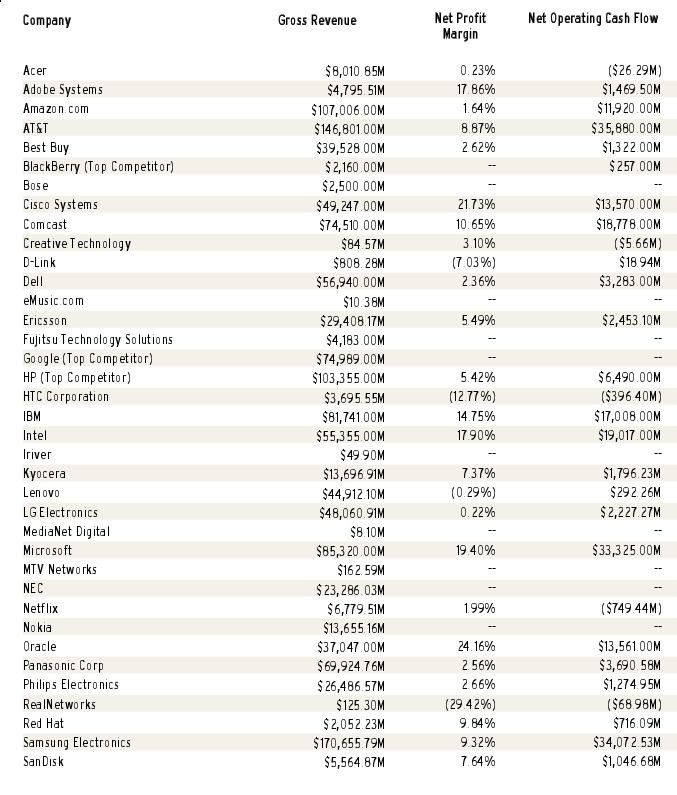
\includegraphics[width=1\textwidth]{competitor1}
    \caption{Taken directly from Hoover~\cite{hoover}}
\end{figure}

\newpage

\begin{figure}[!htb]
  \centering
  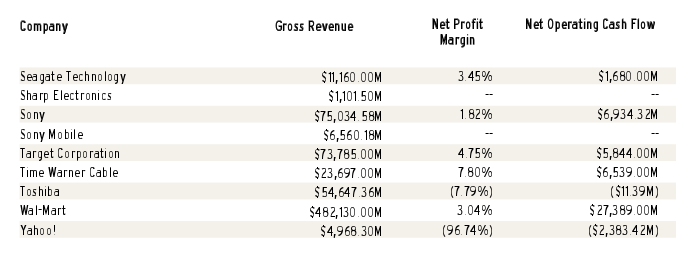
\includegraphics[width=1\textwidth]{competitor2}
    \caption{Taken directly from Hoover~\cite{hoover}}
\end{figure}

\newpage

\printbibliography[
heading=bibintoc,
title={Resources}
]

\end{document}
